\documentclass[]{book}
\usepackage{lmodern}
\usepackage{amssymb,amsmath}
\usepackage{ifxetex,ifluatex}
\usepackage{fixltx2e} % provides \textsubscript
\ifnum 0\ifxetex 1\fi\ifluatex 1\fi=0 % if pdftex
  \usepackage[T1]{fontenc}
  \usepackage[utf8]{inputenc}
\else % if luatex or xelatex
  \ifxetex
    \usepackage{mathspec}
  \else
    \usepackage{fontspec}
  \fi
  \defaultfontfeatures{Ligatures=TeX,Scale=MatchLowercase}
\fi
% use upquote if available, for straight quotes in verbatim environments
\IfFileExists{upquote.sty}{\usepackage{upquote}}{}
% use microtype if available
\IfFileExists{microtype.sty}{%
\usepackage{microtype}
\UseMicrotypeSet[protrusion]{basicmath} % disable protrusion for tt fonts
}{}
\usepackage{hyperref}
\hypersetup{unicode=true,
            pdftitle={Batı Avrupa Ülkelerinde ( İspanya, Portekiz) ve Türkiye'de Kobilere Yönelik Devlet Destekleri ve Destek Önerileri},
            pdfauthor={Selcuk DONMEZ},
            pdfborder={0 0 0},
            breaklinks=true}
\urlstyle{same}  % don't use monospace font for urls
\usepackage{natbib}
\bibliographystyle{apalike}
\usepackage{color}
\usepackage{fancyvrb}
\newcommand{\VerbBar}{|}
\newcommand{\VERB}{\Verb[commandchars=\\\{\}]}
\DefineVerbatimEnvironment{Highlighting}{Verbatim}{commandchars=\\\{\}}
% Add ',fontsize=\small' for more characters per line
\usepackage{framed}
\definecolor{shadecolor}{RGB}{248,248,248}
\newenvironment{Shaded}{\begin{snugshade}}{\end{snugshade}}
\newcommand{\AlertTok}[1]{\textcolor[rgb]{0.94,0.16,0.16}{#1}}
\newcommand{\AnnotationTok}[1]{\textcolor[rgb]{0.56,0.35,0.01}{\textbf{\textit{#1}}}}
\newcommand{\AttributeTok}[1]{\textcolor[rgb]{0.77,0.63,0.00}{#1}}
\newcommand{\BaseNTok}[1]{\textcolor[rgb]{0.00,0.00,0.81}{#1}}
\newcommand{\BuiltInTok}[1]{#1}
\newcommand{\CharTok}[1]{\textcolor[rgb]{0.31,0.60,0.02}{#1}}
\newcommand{\CommentTok}[1]{\textcolor[rgb]{0.56,0.35,0.01}{\textit{#1}}}
\newcommand{\CommentVarTok}[1]{\textcolor[rgb]{0.56,0.35,0.01}{\textbf{\textit{#1}}}}
\newcommand{\ConstantTok}[1]{\textcolor[rgb]{0.00,0.00,0.00}{#1}}
\newcommand{\ControlFlowTok}[1]{\textcolor[rgb]{0.13,0.29,0.53}{\textbf{#1}}}
\newcommand{\DataTypeTok}[1]{\textcolor[rgb]{0.13,0.29,0.53}{#1}}
\newcommand{\DecValTok}[1]{\textcolor[rgb]{0.00,0.00,0.81}{#1}}
\newcommand{\DocumentationTok}[1]{\textcolor[rgb]{0.56,0.35,0.01}{\textbf{\textit{#1}}}}
\newcommand{\ErrorTok}[1]{\textcolor[rgb]{0.64,0.00,0.00}{\textbf{#1}}}
\newcommand{\ExtensionTok}[1]{#1}
\newcommand{\FloatTok}[1]{\textcolor[rgb]{0.00,0.00,0.81}{#1}}
\newcommand{\FunctionTok}[1]{\textcolor[rgb]{0.00,0.00,0.00}{#1}}
\newcommand{\ImportTok}[1]{#1}
\newcommand{\InformationTok}[1]{\textcolor[rgb]{0.56,0.35,0.01}{\textbf{\textit{#1}}}}
\newcommand{\KeywordTok}[1]{\textcolor[rgb]{0.13,0.29,0.53}{\textbf{#1}}}
\newcommand{\NormalTok}[1]{#1}
\newcommand{\OperatorTok}[1]{\textcolor[rgb]{0.81,0.36,0.00}{\textbf{#1}}}
\newcommand{\OtherTok}[1]{\textcolor[rgb]{0.56,0.35,0.01}{#1}}
\newcommand{\PreprocessorTok}[1]{\textcolor[rgb]{0.56,0.35,0.01}{\textit{#1}}}
\newcommand{\RegionMarkerTok}[1]{#1}
\newcommand{\SpecialCharTok}[1]{\textcolor[rgb]{0.00,0.00,0.00}{#1}}
\newcommand{\SpecialStringTok}[1]{\textcolor[rgb]{0.31,0.60,0.02}{#1}}
\newcommand{\StringTok}[1]{\textcolor[rgb]{0.31,0.60,0.02}{#1}}
\newcommand{\VariableTok}[1]{\textcolor[rgb]{0.00,0.00,0.00}{#1}}
\newcommand{\VerbatimStringTok}[1]{\textcolor[rgb]{0.31,0.60,0.02}{#1}}
\newcommand{\WarningTok}[1]{\textcolor[rgb]{0.56,0.35,0.01}{\textbf{\textit{#1}}}}
\usepackage{longtable,booktabs}
\usepackage{graphicx,grffile}
\makeatletter
\def\maxwidth{\ifdim\Gin@nat@width>\linewidth\linewidth\else\Gin@nat@width\fi}
\def\maxheight{\ifdim\Gin@nat@height>\textheight\textheight\else\Gin@nat@height\fi}
\makeatother
% Scale images if necessary, so that they will not overflow the page
% margins by default, and it is still possible to overwrite the defaults
% using explicit options in \includegraphics[width, height, ...]{}
\setkeys{Gin}{width=\maxwidth,height=\maxheight,keepaspectratio}
\IfFileExists{parskip.sty}{%
\usepackage{parskip}
}{% else
\setlength{\parindent}{0pt}
\setlength{\parskip}{6pt plus 2pt minus 1pt}
}
\setlength{\emergencystretch}{3em}  % prevent overfull lines
\providecommand{\tightlist}{%
  \setlength{\itemsep}{0pt}\setlength{\parskip}{0pt}}
\setcounter{secnumdepth}{5}
% Redefines (sub)paragraphs to behave more like sections
\ifx\paragraph\undefined\else
\let\oldparagraph\paragraph
\renewcommand{\paragraph}[1]{\oldparagraph{#1}\mbox{}}
\fi
\ifx\subparagraph\undefined\else
\let\oldsubparagraph\subparagraph
\renewcommand{\subparagraph}[1]{\oldsubparagraph{#1}\mbox{}}
\fi

%%% Use protect on footnotes to avoid problems with footnotes in titles
\let\rmarkdownfootnote\footnote%
\def\footnote{\protect\rmarkdownfootnote}

%%% Change title format to be more compact
\usepackage{titling}

% Create subtitle command for use in maketitle
\providecommand{\subtitle}[1]{
  \posttitle{
    \begin{center}\large#1\end{center}
    }
}

\setlength{\droptitle}{-2em}

  \title{Batı Avrupa Ülkelerinde ( İspanya, Portekiz) ve Türkiye'de Kobilere Yönelik Devlet Destekleri ve Destek Önerileri}
    \pretitle{\vspace{\droptitle}\centering\huge}
  \posttitle{\par}
    \author{Selcuk DONMEZ}
    \preauthor{\centering\large\emph}
  \postauthor{\par}
      \predate{\centering\large\emph}
  \postdate{\par}
    \date{2019-08-20}

\usepackage{booktabs}
\usepackage{amsthm}
\makeatletter
\def\thm@space@setup{%
  \thm@preskip=8pt plus 2pt minus 4pt
  \thm@postskip=\thm@preskip
}
\makeatother

\begin{document}
\maketitle

{
\setcounter{tocdepth}{1}
\tableofcontents
}
\hypertarget{ozet-abstract}{%
\chapter{Ozet-Abstract}\label{ozet-abstract}}

Küçük orta boylu işletmelerin (Kobi) ülke ekonomilerinde ve globalleşen dünyada etki alanı genişlemektedir. Günümüz dünyasında mevcut etki alanıyla küçük orta boylu işletmeler devletler tarafından geliştirilen politikalarla birlikte yeni roller üstlenmekte ve bu rollerin işletmelere getirdiği yenilik ve değişimler analiz edilmektedir. Bu çalışmanın amacı Batı Avrupa ülkelerinde ve Türkiye'de kobilere yönelik destek politikalarına değinilerek, politika belirleyicilere ve uygulayıcılara yol gösterecek önerilerin ortaya atılmasıdır.

Çalışmada Batı Avrupa ülkerinde ve Türkiye'de devlet destekleri, bu ülkelerin ekonomilerinin yapısı ortaya konulacak. Durum değerlendirmesi neticesinde destek modelleri önerilecektir.

\begin{Shaded}
\begin{Highlighting}[]
\NormalTok{Anahtar Kelime }\OperatorTok{:}
\NormalTok{Kobi}
\NormalTok{Devlet Destekleri}
\end{Highlighting}
\end{Shaded}

\hypertarget{intro}{%
\chapter{Giris}\label{intro}}

Son ürünün veya ara mamulün üretilmesi esnasında ana malzemeden yeterli tolerans ve boyutlarda malzemenin en iyi şekilde kesilmesi ve bu malzemenin verimli ve etkin kullanılması endüstride süregelen önemli bir problem olmuştur. Ana malzemeden eniyi sekilde yararlanmak, dolayısıyla malzeme kayıp oranlarını en küçüklemek bu alanda ortaya atılan yaklaşımların en önemli hedefi olmuştur.

Kesme problemleri endustride temin edilen ana malzemeden daha küçük boyutlarda ve yeterli tolerans miktarlarıyla daha küçük malzemelere kesilmesi problemi olarak tanımlanabilir. Bu problem türü endüstride en fazla havacılik, dayanıkli tüketim malzemeleri üreten sanayi kolları, tekstil, mobilya gibi değişik sanayi kollarında ortaya çıkmaktadır.

Bu calısmada dairesel kesme problemi yeni bir yaklaşımla ele alinmış ve bu tür problemlere yeni bir cözum yöntemi geliştirmek hedeflenmistir. Yeni yaklaşımda bir duzleme kesilecek dairesel malzemelerin atanmasında dairesel malzemelerin birbirlerine teğet konumları ele alınarak, daire dilimleri ve bu daire dilimlerini kapsayan çeşitli boy ve ebatlarla olusan ucgenlerin incelenmesiyle atık oranlarını küçükleyecek şekilde bir eniyileme algoritması geliştirmeye çalışılmıştır. Bu yeni yaklaşımla beraber dairesel malzemelerin arasında meydana gelen uçgenlerin incelenmesi bu türden problemlere geometrik olarak daire olmasına rağmen farklı geometrik şekillerle ve tekniklerle incelenebileceği gösterilmeye çalışılmıştır.

Ikinci bölümde dairesel kesme probleminin üçgensel alanların kullanılması yaklasımi aciklanmis ve ayrıntılı olarak ele alınmistir. Ayrıca gelistirilen yaklaşım programlanarak bilgisayar ortamina aktarılmış ve program kodları paylasilmistir. Son olarak yeni yaklaşım küçük boyutlu dairesel atama problemine nasıl uygulandığı gösterilerek sonuçlar değerlendirilmeye çalışılmıştır.

\hypertarget{malzeme-kesme-problemleri}{%
\chapter{MALZEME KESME PROBLEMLERİ}\label{malzeme-kesme-problemleri}}

Sanayide son ürünlerin elde edilmesi için temin edilen ham malzemeler genellikle belirli standart büyüklüklerde ve boyutlarda temin edilebilmektedir, bu hammaddeleri üreten sanayiye girdi sağlayan kuruluşların hammaddeyi ekonomik anlamda üretebilmesi icin ana sebeptir. Dolayısıyla hammadde üreten kuruluşlar malzemenin ekonomik olabilmesi icin belli boyutlarda üretim yapmaktadırlar. Son ürünü üreten işletmelerin bu malzemeleri ana üreticilerden temin edip hammaddeyi kendi malzemelerine uygun olarak tekrar boyutlandırması ve üretim surecine bu şekilde alması gerekmektedir .Malzeme kesme problemlerinin ana konusu ve kaynağı bu noktada meydana gelmektedir. Temin edilen hammaddenin en verimli şekilde nasıl kullanılacağına ilişkin araştırmalar kaynaklarda genel malzeme kesme problemi olarak adlandirilmaktadir.

Bu bölümde malzeme kesme problemleri ile ilgili genel tanim ve kavramlar açıklanmaktadır. Malzeme kesme problemlerinin siniflandirilmasi, kısıtlar ve amaçlar, bu tür malzeme kesme problemlerinin modellenmesi ve kaynaklarda gelistirilen kesme problemlerinin genel tanimi uzerinde durulmaktadir.

\hypertarget{malzeme-kesme-problemlerine-genel-bakis}{%
\section{Malzeme Kesme Problemlerine Genel Bakış}\label{malzeme-kesme-problemlerine-genel-bakis}}

Metal, kağıt, cam, kereste, deri, giyim gibi birçok endüstri alaninda yer tutan bir problem olan malzeme kesme problemi, ''Belirli boy ve ebatlarda temin edilen ana malzemeden, son ürün elde edilmesi icin daha kucuk boyutlarda parcalarin elde edilmesi problemi'' olarak tanimlanabilir.

Malzeme kesme problemleri ana malzemeye küçük kalıpların en küçük atık oranını sağlayacak sekilde nasıl konumlandırılacağı, yerleştirileceğini belirlemesiyle aynı zamanda bir yerlesim planlamasını da bünyesinde barındırmaktadır. Malzeme kesme problemlerinin bir alt kümesi istif problemlerinde ise büyük nesneler boş alan olarak tanimlanmakta ve küçük parçalarla bu boş alanların etkin bir şekilde doldurulmaktadir. Bir diğer malzeme kesme problemi ise, küçük parçalara kesilmesi gereken bküçükyük nesnelere dayanır.

Malzeme kesme problemleri hakkında çok değişik araştırmalar yapılmış ve ayni zamanda çok farklı teknikler geliştirilmiştir. Bunlara bir örnek dik açılı olmayan kesme problemleridir, bu tür problemlerde sipariş parçalarının levha üzerine açılı olarak yerlestirilmesidir. Ayrıca dikdörtgen olmayan şekle sahip parçaların düzenlenmesi problemleriyle de çok sık karşılaşılmaktadır.

Büyük sanayi kuruluslarından elde edilen ve son ürünün elde edilmesi için kullanılan ve kesilmesi gereken malzemelere, \textbf{ana malzeme}, ana malzemeden kesilerek son ürün haline getirilecek olan küçük parçalara ise \textbf{sipariş parçası} denilmektedir. Kesilmesi gereken parçaların ana malzemeye veya hammaddeye nasıl yerleştirileceğini gösteren geometrik modellere ise \textbf{kesme planı} denilmektedir. Sipariş alınan parçaların tümünün elde edilmesini sağlayacak sekilde birden fazla kesme planı hazırlanabilir. Kaynaklarda tek-boyutlu kesme planı, boylarının toplamı ana malzemenin boyunu aşmayan parçaların bir kombinasyonu olarak tanımlanmıştır.

Siparis listesinde bulunmadigi halde kesme planinda kesilecek malzemelerin arasinda degerlendirilemeyen malzemelere ise \textbf{fire} denilmektedir. Malzeme kesme problemlerinde amac fonksiyonu toplam fire miktarinin en kucuklenmesine dayanmaktadir.

\hypertarget{koseli-sekiller}{%
\subsection{Köşeli şekiller}\label{koseli-sekiller}}

Malzeme kesme problemlerinde köşeli şekilli parçaların kesimi ve kesme planlarının hazırlanması önemli bir yer tutmaktadır. Köşeli şekillerin kalıp, sablon vb, kesilmesi islemi özel donanım gerektirmeden, daha kolay bir şekilde yapılabilmektedir. Yerleşim planı tasarımında özellikle düzgün kenarlar, yerleşimi kolaylastırmakta, düşük fireli ve etkin planların kolayca düzenlenebilmesi sağlanmaktadır.

Dik açılı malzeme kesme problemlerinde dikdörtgen parçaların dikdörtgen ana malzeme üzerine eksenleri kesmeyecek, yani paralel olacak şekilde yerleştirilmektedir. Dik açılı olmayan kesme bu tür problemlerde fire oranını azaltabilse bile kesme işleminde kullanılan tezgahlar bu kesimlere izin vermemektedir. Giyotinle kesimde her ardışık kesme işlemi levhanın bir ucundan diğerine uzayacak şekilde kesilmeli ve ayni islem diğer parçalarada uygulanarak parçalar elde edilmelidir.

Iki-boyutlu malzeme kesme problemlerinde kademeli kesme problemlerinin modellenmesi Gomory ve Gilmore'un (1965) çalışmalarıyla başlamıştır. Bu tür kesme islemi ise temel olarak giyotinle kesmenin özel bir durumudur. Bu yöntemle kesme problemlerinde ise ana malzeme alt parçalara ayrılır ve ikinci aşamada bu alt parçalar da ters yönde kesilip daha alt düzeyde parçalar elde edilir. Mobilya sektöründe kullanılan makinelerde bu şekilde kesim yapılır.

Parcaların kesilmesi esnasında bazı kesme problemlerinde parçalarin rotasyonuna izin verilemeyebilir, bu parçaların mukavemet gibi özelliklerinden kaynaklanabilir.

\hypertarget{kesme-problemlerinde-boyut}{%
\subsection{Kesme problemlerinde boyut}\label{kesme-problemlerinde-boyut}}

Kesilecek malzemenin ana malzemenin boyutlarına bağlı olarak bir, bir-buçuk, iki veya üç boyutlu kesmeden söz edilebilmektedir.
Tek-boyutlu kesme: kağıt ruloların ve çubuk malzemelerin kesilmesinde diğer boyutların bir anlamı kalmamaktadır. Gomory ve Gilmore(1961,1963) kağıt rulolara tek-boyutlu malzeme kesme problemini ele almış ve en iyi sonucu veren ilk yontem geliştirilmişlerdir.

\textbf{Bir bucuk-boyutlu kesme}: Bu tür levha uzunluğunun, sonsuz varsayıldığı iki-boyutlu problemlerin özel bir durumudur. Dikdörtgen parçalar çok uzun rulo malzeme uzerine yerleştirileceği zaman bu tür oluşmaktadır.

\textbf{İki-boyutlu kesme}: Rulo saç, kumaş ve deri gibi levhalardan kesilecek parçaların bu ana malzemelere toplam fireyi en küçükleyecek şekilde dizilmesini ele almaktadır.

\textbf{Üc-boyutlu kesme}: Aynı veya farklı biçimlerdeki n adet cismin sabit bir hacme toplam yerlesim hacmini en küçükleyecek şekilde yerleştirilmesini amaçlamaktadır.

Üç-boyutlu kesme problemlerinde geometrik olarak düzgün olmayan şekillerle karşılasilsa bile, düzensiz parçaların kesimine yönelik bir yöntem geliştirilememiştir. Zaten böyle parcaların kesilebilmesi için öncelikle bu düzgün olmayan şekilleri kapsayan parcaların kesilmesi daha sonra elde edilen parçaların bir çeşit oyma işleminden geçirilmesi ve yeniden duzeıılenmesiyle mümkün olacağı düşünülmektedir.

\hypertarget{kesme-problemlerinin-siniflandirilmasi}{%
\section{Kesme Problemlerinin Siniflandirilmasi}\label{kesme-problemlerinin-siniflandirilmasi}}

Malzeme problemlerinin gerçek hayat şartlarında çeşitli boyutları ortaya çıkmıstır. Benzer mantıksal yapılara sahip bu malzeme kesme ve istif problemleri çeşitli adlara sahiptir. Bunlar; malzeme kesme ve fire kaybı problemleri, kutu yerlestirme, serit yerlestirme, vektör yerleştirme, sırt çantası, araç yukleme gibi adlarla da anilmaktadirlar.

Değisik turdeki iki-boyutlu kesme problemleri kaynaklarda oldukça önemli bir yer tutmaktadır. Bu tür problemler; ana malzemeden küçük parçaların kesilmesi olarak, veya küçük parcaların ana malzemeye yerleştirilmesi problemi olarak ele alınabileceği için aynı zamanda bir yerleşim problemidir.

Malzeme ve boşluk arasındaki ikili ilişkiden yola çıkılarak, kesme ve yerleştirme problemleri arasında güçlü bağa dikkat çekilmiştir. Bu bakış açısıyla, yerleşim problemlerinin, küçük parçaların büyük nesneye yerleştirilmesi olarak düşünülebileceğini; tersi durumda ise malzeme kesme problemlerinin büyük nesnelerin daha küçük nesnelere bölünmesi olarak tanımlanması arasındaki yakın ilişkiye dikkat çekilmiştir.

Malzeme kesme problemlerinin yapısı kesilecek veya yerleştirilecek parçaların geometrik özelliklerine göre değişmektedir. Malzeme kesme problemlerini bu yönüyle düzenli ve düzensiz şekilli malzeme problemi olarak ikiye ayırmak mümkündür. Malzeme kesme problemlerinde geometrik olarak düzgün yapiya sahip malzemelerin kesilmesi işlemi düzenli şekilli malzeme kesme problemi olarak adlandırılırken, düzensiz şekilli kesme problemlerinde özellikle problemin modellenmesi oldukça güç olmaktadır.

\hypertarget{boyutlarina-gore-gruplama}{%
\subsection{Boyutlarına göre gruplama}\label{boyutlarina-gore-gruplama}}

Malzeme kesme problemlerinin en önemli özelliği boyutudur ve bu özelliği ayırıcı bir özellik teşkil etmektedir. Bu problemlerde doğrultu sayısı kesme probleminin boyutunu vermektedir. Kesme problemlerinin ağırlık veya zaman gibi boyutlar içermesi durumunda problem daha fazla boyut kazanabilmektedir.

\hypertarget{talep-turune-gore-siniflandirma}{%
\subsection{Talep türüne göre siniflandirma}\label{talep-turune-gore-siniflandirma}}

Her parçaya ait talep, o parca için kesilecek toplam miktarla sınırlandırılmakta ise kısıtlı tersi durum için ise problem kısıtsız malzeme kesme problemi olarak adlandırılmaktadır. Kısıtlı malzeme kesme problemlerinde bazı parçalara ait talep miktarları, o parcanin bir levhadan kesilebilecek toplam parça sayısından küçük olabilmektedir.

\hypertarget{kesme-problemlerinin-kisitlari}{%
\section{Kesme Problemlerinin Kisitlari}\label{kesme-problemlerinin-kisitlari}}

Malzeme kesme problemleri talep türüne göre kısıtsız ya da kısıtlı olarak adlandırılabilmektedir. Ilk türdeki problemlerde sipariş parçaları için talep miktarı sınırlı olmayıp, mümkün olan en büyük sayıda parçanın kesilmesi amaçlamaktadır.
Kısıtlı olan ikinci problem türünde ise sipariş parçalarına ait talep miktarları bellidir ve bu miktarlardan daha fazla kesim işlemine izin verilmemektedir.

Malzeme kesme problemlerinde genellikle iki tür kısıttan söz edilmektedir. Giyotin kısıtı her kesme islemi sonunda iki dikdörtgen parça elde etme gereği, diğeri her parçanın yönünün sabit olmasi l uzunluğunda ve l genişliğindeki parçadan farklı
olması gereğidir.

Giyotinle kesme cam, mobilya gibi bir çok endüstri dalında, kesme işleminin teknolojik yönüyle ihtiyac duyulmaktadır. Parçanın döndürülmesine izin verilmemesi ise örneğin parçanin desenli bir yapıda olmasından kaynaklanmaktadır. Gerçek hayat problemlerinde, düz malzemelerin kesilmesinde ve çoğu yerleştirme işleminde, daha iyi yerlesimler elde edilmesi icin parçaların döndürülmesine izin verilebilir.

\hypertarget{kesme-problemlerinde-benimsenebilir-amaclar}{%
\section{Kesme Problemlerinde Benimsenebilir Amaçlar}\label{kesme-problemlerinde-benimsenebilir-amaclar}}

Malzeme kesme problemlerinde her ana malzeme ve sipariş parçasına bir değer atanmaktadır. Temel olarak fire miktarının en küçüklenmesi amaçlandığı için bu değer parçanin alanına esit olarak belirlenmektedir. Ancak uzun süre depoda bekleyen bir ana malzemenin değerinin azaltılması veya acil öncelikli bir parçanın değerinin artırılması durumlarını modele yansıtmak amacıyla bu değerin bir katsayıyla çarpılması kullanıcılar tarafından talep edilebilmektedir.

Malzeme kesme problemlerinde toplam firenin en küçüklenmesi olan amaç fonksiyon, kullanılan her parcadan elde edilecek faydanın o parçanın alanıyla orantılı olarak belirlenmesi durumunda bir en buyükleme problemine dönüştürülebilir.

\citep{xie2015}
\citep{xie2016}
\citep{xie2016}
\citep{xie2017}
\citep{xie2018}
\citep{xie2019}

\hypertarget{ucgensel-alanlar-ve-dairesel-kesme-problemlerinin-cozumu-icin-gelistirilen-yaklasim}{%
\chapter{ÜÇGENSEL ALANLAR ve DAİRESEL KESME PROBLEMLERİNiN ÇÖZÜMÜ İÇİN GELİSTİRiLEN YAKLASIM}\label{ucgensel-alanlar-ve-dairesel-kesme-problemlerinin-cozumu-icin-gelistirilen-yaklasim}}

Bu calışmada, dairesel kesme probleminin çözümü için daireler arasında oluşan üçgensel alanların incelenmesine yönelik yeni bir yaklaşim incelenmiştir.

Geliştirilmeye çalışılan algoritmanın temelleri öncelikle ana malzemenin tek olduğu ve fireyi en küçükleyecek şekilde kümelenmiş dairelerin verilen listede kesilmek istenen yarı çaplarin en uygun olanının secilmesi ve atanması işlemiyle gerçekleşmektedir. Eldeki malzeme listesinde en uygun yarıçaplı çember atanmis çemberlerle ikili olarak ele alınmakta ve atık kısım üçerli çember alanlarının toplamına bölünmesi yani toplam bir oran en küçüklemesi yaklaşımıyla uygun yarıçaplı çemberi seçmektedir.

Başlangıç olarak bu yeni algoritmada üç daire uzerinde durulmus ve çesitli yarıçaplara sahip dairelerin nasıl bir araya geldikleri ve kümelenmelerde atik oranlari incelenmistir. Dolayısıyla bu üçlü varyasyonların geometrik özellikleri çikartilmis ve bu üçgen yardımıyla diğer malzemelerin nasıl atanacağı konusunda fikir edinilmeye çalışılmıştır.

Öncelikle temel olarak üç dairenin nasil bir araya geldigi ve bunlara iliskin geometrik formüller ve hesaplamalar gösterilecektir. \textbf{Şekil 1.1} de genel olarak üç dairenin nasil bir araya geldigi ve incelenmesi gereken ortadaki üçgen gösterilmiştir.

Burada önemli olan bir nokta ise bir araya gelecek bu dairelerin birbirleri üzerine çakışmadan ve aralarında herhangi bir boşluk bulunmadan nasıl yerleştirilebileceği problemidir. Bu problem üçgenin iç açılarının bulunması ve bu iç açıların toplamının l80 dereceye ulasması halinde algoritma denenen yarıçapı hafızada tutmaktadır. Dolayısıyla denenen yarıcap ücgenin iç açıları toplamini sağlamıyorsa atanacak yarıçap elenmektedir. Böylece atama esnasında oluşacak çakışma ve arada boşluk bulunması ve bunların tekrar moduller yardımıyla düzenlenmesi işlemini çözüm yöntemiyle aşmakta ve bunun için zaman harcamamaktadır. \textbf{Şekil 1 . 2}' de dairelerin arasindaki üçgen ve bu üçgenin iç açilarinin nasil nasıl hesaplandığı görülmektedir.

\begin{figure}

{\centering 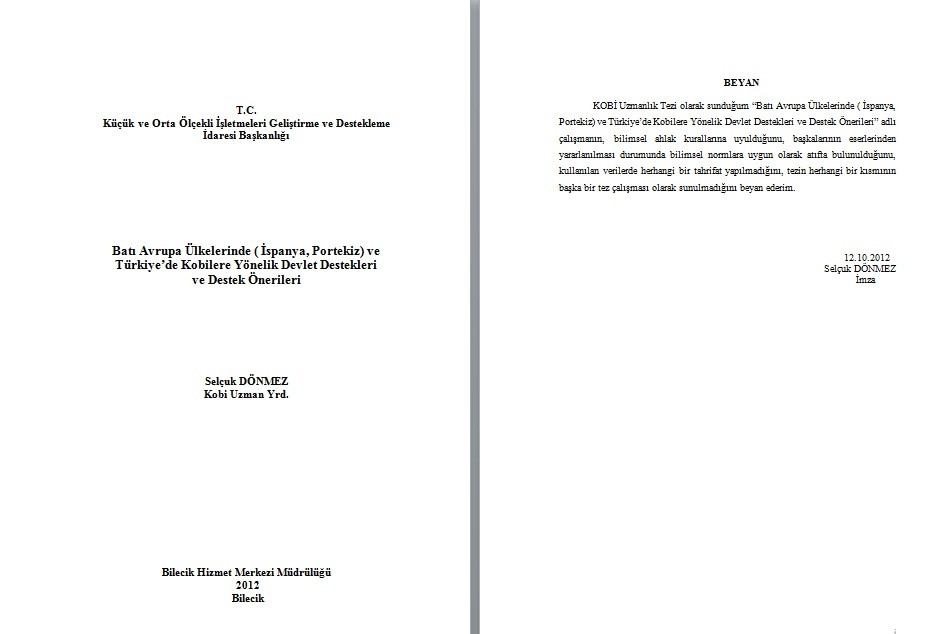
\includegraphics[width=0.7\linewidth]{bookdown/figure/1} 

}

\caption{Sekil 1.1 Acilar ve Geometrik Cizimler}\label{fig:pressure}
\end{figure}

Daireler arasında kalan üçgenlerin oluşturacağı iç açların yani α,β, ⌀ açıları formül yardımıyla hesaplanacak ve bu açılarının arcsinleri alınarak derece cinsinden olusan açıların sayısal değerleri elde edilmiş olacaktır. Burada üçgenin iç açılarının sinüslerinin bulunmasıyla \textbf{Alan = L/2sina (rt+r2)x(rl+r3)} formülüyle oluşan üçgen alanı tespit edilecektir. Ayrıca üçgenin kenar açıları daire dilim merkezleri olduğu için atık alanı hesaplanmasında üçgen alanından bu daire dilimlerinin çıkarılmasıyla ortaya çıkan atık alani belirlenmis olacaktır. Bilgisayar programında bu atık oranı ele alinan üçlü dairenin alanı toplamina bölunmesiyle oran tespit edilecek ve seçeneklerin denenmesi ve en düşük atık oranını sağlayan yarıçapın hafızaya alınıp düzleme atanması işlemiyle saglanacaktir.

\begin{figure}

{\centering 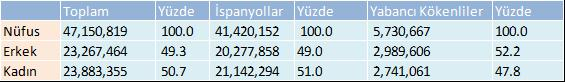
\includegraphics[width=0.7\linewidth]{bookdown/figure/2} 

}

\caption{sekil 1.2 Ucgen  ve Ic aci hesaplari}\label{fig:pressure1}
\end{figure}

Bilgisayar programında en iyi yarıçap bulunduktan sonfa bu çemberin ne tarafa ve nereye çizileceği problemini yine geometrik olarak iki noktası ve kenar uzunlukları belli olan ücgenin ücüncü kösesini daireler yardımıyla geometrik açıdan çözebiliyoruz. Bilgisayar programında bu noktayı tespit edebilmek için kırmızı renkli daireler çizilmekte ve bu dairelerin kesişim noktasının kullanıcı tarafindan belirlenmesiyle bu probleme geçici bir çözüm bulunmuştur.

Örnek olarak r1:5OO, r2:900 ve r3:85O daireleri başlangıç olarak yerlestirildiginde listbox 'tan bir en iyi değer aranmaktadır. Bir yerleştirmenin program yardımıyla nasıl çözüldüğü Şekil l.3 yardımıyla gösterilmiştir.

\hypertarget{sonuc-ve-oneriler}{%
\chapter{SONUÇ VE ÖNERİLER}\label{sonuc-ve-oneriler}}

Dairesel kesme problemi icin geliştirilen bu algoritma ve yeni yaklaşım henüz belli sayıda dairelerin atanması islemini etkin olarak gerçekleştirmektedir. Dolayısıyla daha fazla cemberin etkin bir şekilde yerleşiminin gerçekleştirilmesi için atanacak çemberlerin yerleşiminde kullanıcının noktayı belirlemesini ve pivot çemberler yardımıyla atama yapmasi yerine bu soruna analitik bir yaklaşım ve yeni bir yöntem bulunması kaçınılmazdır.

Geliştirilmeye çalışılan yeni yaklaşım dairesel malzeme kesme problemleri için çesitli tekniklerle uygulanarak daha etkin çözümler elde edilebileceği düşünülmektedir. Örnek olarak bu yeni atama yaklaşımının genetik algoritmalar teknikleriyle kullanılması, veya çemberlerin yan taraflarına eklenecek çemberler araştırılırken bir çeşit dal sınır tekniğiyle bu tür problemlerin daha fazla sayıda çember yerleştirilmesinde kullanılması düşünülebilir. Bu çalışmada bu tür problemlerin daha farklı bir şekilde nasıl ele alınabileceği arastirilmiş ve bu türden problemlerin geometrik özellikleri değerlendirilerek yeni bir yaklaşım geliştirilmeye çalışılmıştır.

Visual Basic de yazılan bu program geliştirilerek cad yazılımlarıyla entegre hale getirilmesi halinde sanayiye önemli katkısı olabileceği düşünülmektedir. Bu programın geliştirilerek ve daha etkili çözümlemelerle daha iyi kodlanabileceği ve genetik algoritma gibi tekniklerle daha iyi sonuçlar elde edileceği düşünülmektedir.

\hypertarget{visual-basic-6-ekran-goruntuleri}{%
\chapter{Visual Basic 6 Ekran Goruntuleri}\label{visual-basic-6-ekran-goruntuleri}}

\begin{figure}

{\centering 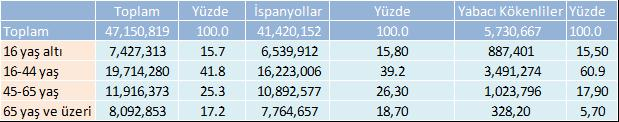
\includegraphics[width=0.5\linewidth]{bookdown/figure/3} 

}

\caption{ Baslangic Yerlesimi}\label{fig:pressure3}
\end{figure}

\begin{figure}

{\centering 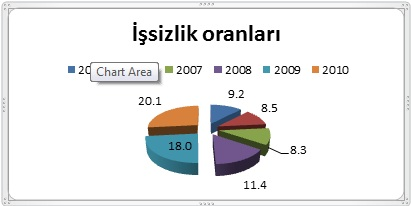
\includegraphics[width=0.5\linewidth]{bookdown/figure/4} 

}

\caption{ Koordinatlarin Isaretlenmesi}\label{fig:pressure4}
\end{figure}

\begin{figure}

{\centering 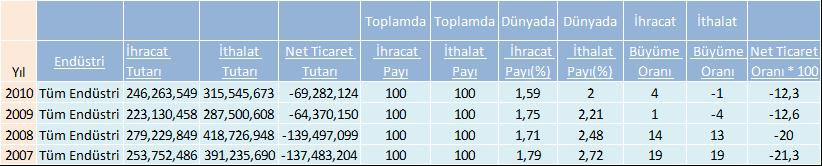
\includegraphics[width=0.5\linewidth]{bookdown/figure/5} 

}

\caption{ Birinci Cemberin Atanmasi}\label{fig:pressure5}
\end{figure}

\begin{figure}

{\centering 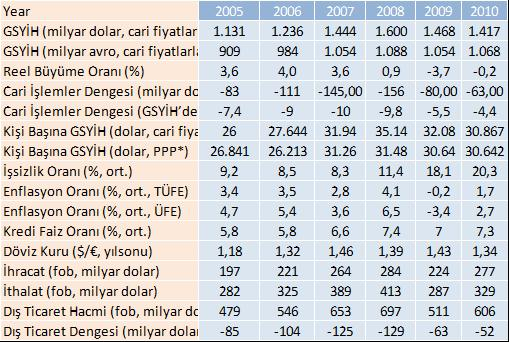
\includegraphics[width=0.5\linewidth]{bookdown/figure/6} 

}

\caption{ Uygun Bolgenin Isaretlenmesi}\label{fig:pressure6}
\end{figure}

\begin{figure}

{\centering 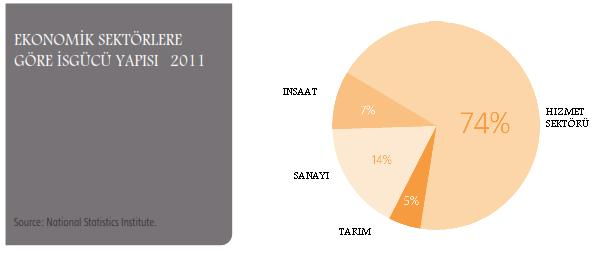
\includegraphics[width=0.5\linewidth]{bookdown/figure/7} 

}

\caption{ Ikinci Cemberin Atanmasi}\label{fig:pressure7}
\end{figure}

\begin{figure}

{\centering 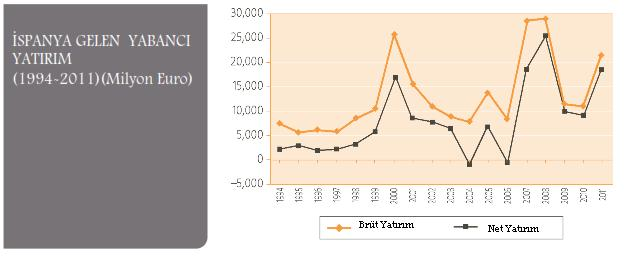
\includegraphics[width=0.5\linewidth]{bookdown/figure/8} 

}

\caption{ Uygun Bolgenin Isaretlenmesi}\label{fig:pressure8}
\end{figure}

\begin{figure}

{\centering 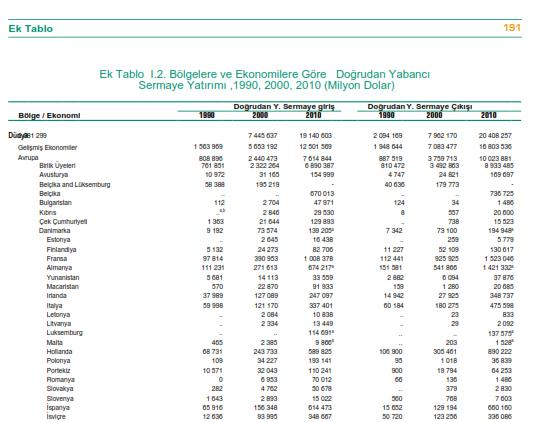
\includegraphics[width=0.5\linewidth]{bookdown/figure/9} 

}

\caption{ Ucuncu Cemberin Atanmasi}\label{fig:pressure9}
\end{figure}

\begin{figure}

{\centering 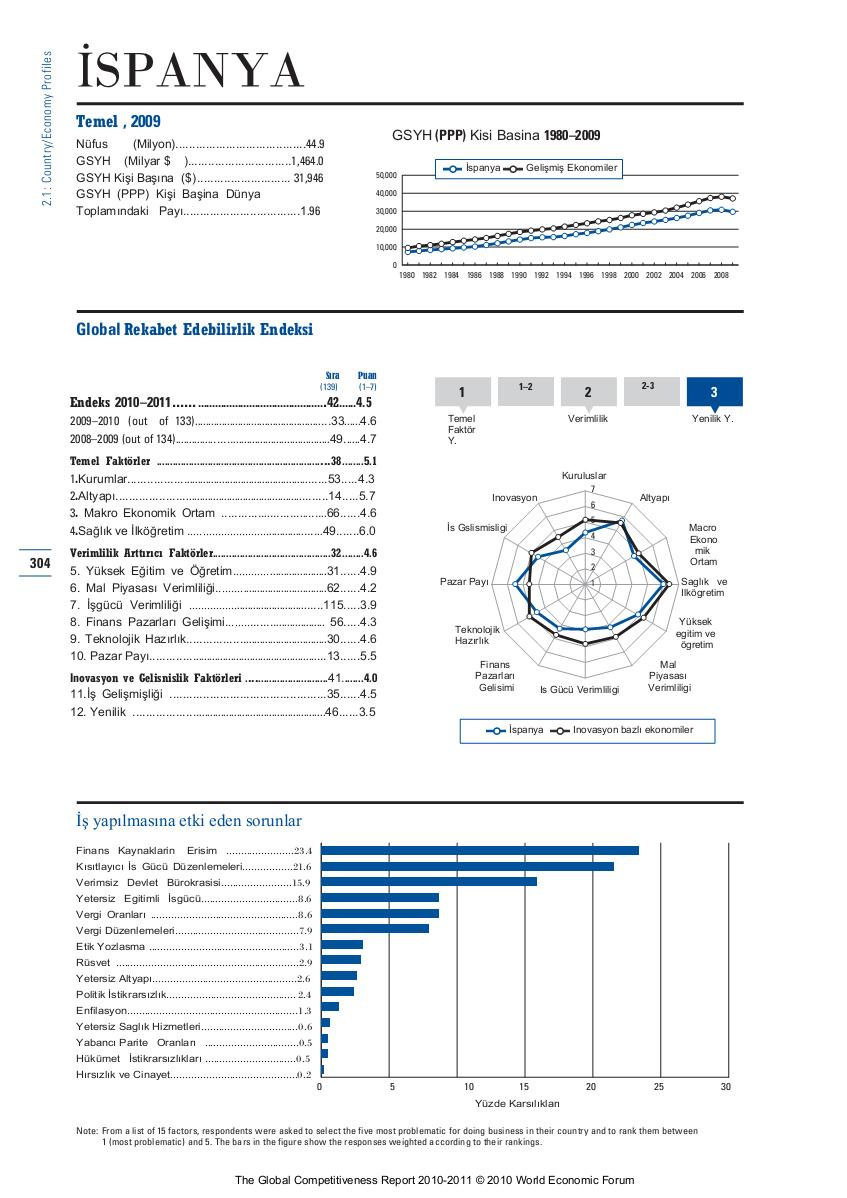
\includegraphics[width=0.5\linewidth]{bookdown/figure/10} 

}

\caption{sekil 1.3h Istatistik Hesaplari}\label{fig:pressure10}
\end{figure}

\hypertarget{ekler}{%
\chapter{Ekler}\label{ekler}}

EK-1 Visual Basic Program Kodları \(\\\)
Option Explicit\(\\\)
Dim matris(1To 10, 1 To 2) As Integer\(\\\)
Diın curx, cury As Integer\(\\\)
Dim dizi . soıı\_basamak As Integer\(\\\)
Diın toplam As Double\(\\\)
Dim artık\_0, artık\_l , artık\_2, artık\_ilk As Dorıble\(\\\)
Diın alanlar1, alanlar2, alanlar3 As Double\(\\\)
Dim açılar(2) As String\(\\\)
Dim gerçek\_açılar(2) As String\(\\\)
Dim gerçek açılar1(2) As String\(\\\)
Diın dolu\_alan As Currency\(\\\)
Dim atıl As Currency\(\\\)
Dim enk\_atık oranı(2) As Currency\(\\\)
Dim kenar\_atık oranı(2) As Double\(\\\)
Dim enkucuk As Currency\(\\\)
Diırr alfa, beta, teta As Double\(\\\)
Dim q,w, e As Integer\(\\\)
Dim X, Y As Integer\(\\\)
Dim kenar, kenar1, kenar2 As Currency\(\\\)
Diın a, b, c As Double\(\\\)
Dim koor(), j As Integer\(\\\)
Dim artık\_baslangıc As Double\(\\\)
Private Sub Command 1 \_Click()\(\\\)
Dim sayac As Integer\(\\\)
Dim t1(1) As String\(\\\)
For sayac:0 To 1\(\\\)
tl(sayac) : InPutBox("kirmizı çemberlerin kesişim noktasmı işaretleyiniz!,,)\(\\\)
Next sayac\(\\\)
If son\_basamak=kenar\_atık oranı(l) Then\(\\\)
If enk atık\_oranı(O) \textless{} enk atık\_orani(2) Then\(\\\)
Circle (matris(l, l), matris(1,2)), a\(\\\)
Circle (matris(2, l), matris(2, 2)), b\(\\\)
Circle (matıis(3, 1), matris(3 ,2)), c\(\\\)
Circle (matris(4, 1), matris(4, 2)), son\_basamak\(\\\)
Circle (matris(l, 1), matris(1,2)), a + kenar\_atık\_orani(0), QBColor(15)\(\\\)
Circle (matris(2, 1), matris(2 ,2)),b + kenar\_atık\_orani(0),QBColor(15)\(\\\)
Circle (t1 (0), t1(1)), kenar\_atık\_oranı(0)\(\\\)
Else\(\\\)
Circle (matris( 1 , 1), matris (1, 2)), a\(\\\)
Circle (matris(2, 1), ınatris(2, 2)), b\(\\\)
Circle (matris(3, 1), matris(3 ,2)), c\(\\\)
Circle (matris(4, 1), matris(4, 2)), son\_basamak\(\\\)
EK-2 Visual Basic Program Kodları(devam)\(\\\)

Circle (matris(2, l ), matris(2, 2)), b + kenar\_atık\_oranı(2), QBColor( 1 5)\(\\\)
Circle (matris(3, 1), matris(3 ,2)), c + kenar\_atık\_oranı(2), QBColor(15)\(\\\)
Circle (t1 (0), t1 ( 1)), kenar\_atık\_oranı(2)\(\\\)
Eııd If\(\\\)
End If\(\\\)

If son\_basamak = kenar\_atık oranı(0) Then\(\\\)
if eıık\_atık\_oranı(l) \textless{} enk\_atık\_oranı(2) Then\(\\\)
Circle (matris( 1 , l ), ınatris (1, 2)), a\(\\\)
Circle (ınatris(2, 1), matris(2, 2)), b\(\\\)
Circle (matris(3, 1), matris(3 ,2)), c\(\\\)
Circle (ınatris(4, 1), matris(4, 2)), son\_basamak\(\\\)
Circle (matris(1, 1), matris(1,2)), a + kenar\_atık\_oranı( 1), QBColor(1 5)\(\\\)
Circle (matris(3, 1), matris(3 ,2)), c + kenar\_atık\_ oranı( 1), QBColor(1 5)\(\\\)
Circle (t1(0), tl(1)), kenar\_atık\_oranı(l)\(\\\)
Else\(\\\)
Circle (matris(l, l), matris(1,2)), a\(\\\)
Circle (matris(2, 1), matris(2 ,2)),b\(\\\)
Circle (matris(3. 1), matris(3 ,2)), c\(\\\)
Circle (matris(4, 1), matris(4, 2)), son\_basamak \(\\\)
Circle (matris(2, 1), matrİs(2, 2)), b+ kenar\_atık\_oranı(2), QBColor(l 5)\(\\\)
Circle (matris(3, 1), matris(3 ,2)), c + kenar\_atık\_oranı(2),QBColor(15)\(\\\)
Circle (t1(0), tl (l )), kenar\_atık\_oranı(1)\(\\\)
End If\(\\\)
End If\(\\\)
If son\_basamak = kenar\_atık oranı(2) Then\(\\\)
If enk\_atık\_oranı( 1 ) \textless{} enk\_atık\_oraru(0) Tlren\(\\\)
Circle (matris(1, 1), matri(1,2), a\(\\\)
Circle (ınatris(2, 1), matris(2, 2)), b\(\\\)
Circle (matris(3, l), matris(3 ,2), c\(\\\)
Circle (matris(4, 1), matris(4,2)), son\_basamak\(\\\)
CircIe (ınatris( l . 1), matris (1.2), a + kenar\_atık\_oranı(1 ), QBCoIor( l 5)\(\\\)
Circle (matris(3, 1), matris(3 ,2)), c +kenar\_atık\_oranı(1), QBColor(15)\(\\\)
Circle (t1 (0), t1 (1 )), kenar\_atık\_oranı(1)\(\\\)
Else\(\\\)
Circle (matris(1, 1), matris(1 ,2)), a\(\\\)
Circle (matris(2. 1 ), matris(2, 2)), b\(\\\)
Circle (matris(3, 1), matris(3 ,2)), c\(\\\)
Circle (matris(4, 1), matris(4, 2)), son\_basamak\(\\\)
Circle (matris( 1, 1 ), matris (1, 2)), a+ kenar\_atık\_oranı(0), QBColor( 1 5)\(\\\)
Circle (matris(2, 1), matris(2 ,2)),b + kenar\_atık\_ oranı(0);, QBColor( 1 5)\(\\\)
Circle (tl(0), t1( 1)), kenar\_atık\_oranı(0)\(\\\)
EK-3 Visual Basic Program Kodları(devam)\(\\\)

End If\(\\\)
End If\(\\\)
End Sub\(\\\)

Private\_Sub\_Command2\_Click()\(\\\)
Dim t(l) As String\(\\\)
For j :0 To 1\(\\\)
t(i) : InputBox(``kırmızı çemberlerin kesişiminin ilkolarak x sonra y koordinatını\(\\\) giriniz'')\(\\\)
Next j\(\\\)
If enk\_atık oranı(0) \textless{} enk\_atık\_oranı( 1 ) And enk\_atık\_oranı (0) \textless{} \(\\\) enk\_atık\_oranı(2) Then\(\\\)
Circle (matris(1, 1), ınatris(1,2)), a +son\_basamak, QBColor(15)\(\\\)
Circle (matris(2, 1), matris(2, 2)), Val(b+son\_basamak) QBColor(15)\(\\\)
End If\(\\\)
If enk atık\_oranı(l) \textless{} enk atık\_oranı(0) And enk\_atık\_ oranı(1) \textless{} enk\_atık\_ oranı(2)\(\\\) Then\(\\\)
Circle (natıis(3, 1), ınatris(3,2)),( c +son\_basamak), QBColor(15) \(\\\)
Circle (matris(1, 1), ınatris(1,2)), son\_basamak+ a), QBColor(15)\(\\\)
End If\(\\\)
If enk atık\_oranı(2) \textless{} enk atık\_oranı(1) And enk\_atık\_ oranı(2) \textless{} enk\_atık\_ oranı(0)\(\\\) Then\(\\\)
Circle (matris(2, 1), matris(2,2)), (b +son\_basamak), QBColor(l5) \(\\\)
Circle (matris(3, 1), matris(3 ,2)), (c + son\_basamak), QBCotor(l5)\(\\\)
End If\(\\\)
Circie (t(0), t(1)), son\_basamak\(\\\)
nıatris(4, l) : CıırrentX\(\\\)
matris(4, 2): CurrentY\(\\\)
End Sub \(\\\)

Private Sub Commaııd4\_Click()\(\\\)
If son\_basamak=kenar\_atık\_oranı(1) Then\(\\\)
If enk\_atık oraııı(O) \textless{} enk\_atık\_oranı(2) Then
Circle (ırratris(2, 1), matris(2 ,2)), b+ kenar\_atık\_oranı(2), 500\(\\\)
Circle (matris(3, 1), matris(3 ,2)), c + kenar\_atık\_oranı(2),500\(\\\)
Else\(\\\)
Circle (matris(l, 1), matris (1, 2)), a +kenar\_atık\_oranı(0), 500\(\\\)
Circle (matris(2, 1), matris(2 ,2)),b + kenar\_atık\_oranı(0), 500\(\\\)
End If\(\\\)
End If\(\\\)
EK-4 Visual Basic Program Kodları(devam)\(\\\)

If soıı\_basamak =kenar\_atık\_oranı(0) Then\(\\\)
If enk\_atık\_oranı (l) \textless{} enk\_atık\_oranı(2) Then\(\\\)
Circle (matris(2, 1), matri(2 ,2)),b+ kenar\_atık\_oranı(2), 500\(\\\)
Circle (ııatıis(3, 1), matris(3 ,2)), c + kenar\_atık\_oranı(2),500\(\\\)
Else\(\\\)
Circle (matris( 1 , 1), matris (1, 2)), a+ kenar\_atık\_oranı ( 1), 500\(\\\)
Circ-le (matris(3, l), matris(3 ,2)), c + kenar\_atık.\_oranı(1), 500\(\\\)
End If\(\\\)
End If\(\\\)
If son\_basamak= kenar\_atık\_oranı(2) Then\(\\\)
If enk\_atık\_oranı(1) \textless{} enk\_atık\_oranı(0) Then\(\\\)
Circle (matris(1, 1), matris(1,2)), a + kenar\_atık\_oranı (0), 500\(\\\)
Circle (matris(2, 1), matris(2 ,2)),b + kenar\_atık\_oranı(0), 500\(\\\)
Else\(\\\)
Circle (matris(l, 1), matris (1,2)), a + kenar\_atık\_oranı(1), 500\(\\\)
Circle(matris(3, 1), matris(3 ,2)), c + kenar\_atık\_oranı(1), 500\(\\\)
End if\(\\\)
End If\(\\\)
End Sub\(\\\)

Private Sub Command5\_Click()\(\\\)
Dim t2(1) As String\(\\\)
Dim sayac As Integer\(\\\)
For sayac=0 To 1\(\\\)
t2(sayac) : InputBox("kirmizi çemberlerin kesişim ıroktasını işaretleyiniz!)\(\\\)
Next sayac\(\\\)
If son\_basamak=kenar\_atık oranı(1) Then\(\\\)
If enk\_atık\_oranı(0) \textless{} enk\_atık\_oranı(2) Then\(\\\)
Circle (matris(2, l ), matris(2, 2)), b + keııar\_atık\_oranı(2), QBColor(15)\(\\\)
Circle (matris(3, 1), matris(3 ,2)), c+ keııar\_atık\_oranı(2), QBColor(15)\(\\\)
Circle (t2 (0), t2 (1)), kenar\_atık\_oranı (2 )\(\\\)
Else\(\\\)
Circle (matris(l, 1), matris(1,2)), a +kenar\_atık oranı(0), QBColor(l5)\(\\\)
Circle (ııatris(2, l ), matris(2, 2)), b + kenar\_atık oranı(0), QBColor(15)\(\\\)
Circle (t2(0),t2(1)), kenar\_atık\_oranı(O) \(\\\)
End If\(\\\)
End If\(\\\)
If son\_basamak= kenar\_atık\_oranı(0) Then\(\\\)
If enk\_atık\_oranı ( 1 ) \textless{} enk\_atık\_oranı (2) Then\(\\\)
Circle (matris(2, 1), matris(2, 2)), b+ kenar\_atık\_oranı(2), QBColor(l5)\(\\\)
Circle (matris(3, 1), matris(3 ,2)), c + kenar\_atık\_oranı(2), QBColor(l5) \(\\\)
EK-5 Visual Basic Program Kodları(devam)\(\\\)

Circle (t2(0), t2(1)), kenar\_atık\_oraıı(2)\(\\\)
Else\(\\\)
Circle (matris (1,1), matris (1, 2)), a + kenar\_atık\_oranı( 1 ), QBColor(1 5)\(\\\)
Circle (matris(3, 1), matris(3 ,2)), c + kenar\_atık \_oranı(1), QBColor(l5)\(\\\)
Circle (t2(0), t2(l)), kenar\_atık oranı(1)\(\\\)
End If\(\\\)
End If\(\\\)
I f son\_basamak= kenar \_atık\_oranı (2) Then\(\\\)
If enk\_atık\_oranı(l) \textless{} enk\_atık\_oranı (0) Then\(\\\)
Circle (matris(l, 1), matris(1,2)),a + kenar\_atrk \_oranı(O), QBCotor( 1 5)\(\\\)
Circle (matris(2, l), matris(2 ,2)),b + kenar\_atık \_oranı (O), QBColor(15)\(\\\)
Circle (t2 (0), t2(1)), kenar\_atık\_oraııı(0 )\(\\\)
Else\(\\\)
Circle (matris(l, 1), matris(1,2)), a + kenar\_atık\_oranı(1), QBColor(l5)\(\\\)
Circle (matris(3, 1), matris(3 ,2)), c + kenar\_atık\_oranı(1), QBColor(l5)\(\\\)
Circle (t2(0), t2(1)), kenar\_atık oranı(l)\(\\\)
End If\(\\\)
End If\(\\\)
End Sub\(\\\)

Private Sub Command6\_Click() \(\\\)
Dim alan\_oranı As Double\(\\\)
Label11.Caption = artık\_0 + artık\_l + artık\_2 + artık\_baslangıc\(\\\)
alan\_oranı =3.145 * (kenar\_atık oranı(0) \^{} 2 + kenar\_atık oranı(1) \^{} 2+\(\\\)
kenar\_atik\_oranı(2) \^{}2+a \textsuperscript{2+b}2+\textsuperscript{c}2)\(\\\)
Label12.Caption : Val(artık\_0 + artık\_1+ artık\_2 +artık\_baslangıc)/alan\_oranı\(\\\)
End Sııb\(\\\)

Private Srıb Forııı load()\(\\\)
Forml.Show\(\\\)
Forml.Height: 10000\(\\\)
Forml.Width : 10000\(\\\)
Diıır yarıcap\(\\\)
Dim i As Integer\(\\\)
yarıcap =Array(l 00, 700, 450, 200, 900, 850, 500, 600, 130, 140, 200, 95)\(\\\)
For i=0 To 11\(\\\)
Listl.Addltem(yarıcap(i))\(\\\)
Next i\(\\\)
Hesapla\(\\\)
cember\_ekle\(\\\)

EK-6 Visual Basic Program Kodları(devam)\(\\\)

End Sub\(\\\)
Private Sub cember\_ekle()\(\\\)
Dinr içlerO, içlerl , içler2 İs Double\(\\\)
Dim e As Integer\(\\\)
Diın p, s As Double\(\\\)
Dim k, l, u As Integer\(\\\)
p =(Val(a) + Val(b) + Val(c))\(\\\)
s=(2 \emph{Sqr(p} a * b * c))\(\\\)
kenar=(Val(a) +c) * (Val(a) +b)\(\\\)
kenar1=(Val(a) +c) * (Val(b) +c)\(\\\)
kenar2=(Val(b) +c) * (Val(b) +a)\(\\\)
açılar(0)=s/kenar\(\\\)
açılar(1)=s/kenar1\(\\\)
açılar(2)=s/kenar2\(\\\)
içler0= (açılar(O) / Sqr((-açılar(0) \^{}2) + 1)) \(\\\)
içler1= (açılar(1) / Sqr((-açılar(1) \^{}2) + 1)) \(\\\)
içler2= (açılar(2) / Sqr((-açılar(2) \^{}2) + 1)) \(\\\)
gerçek açılar(0) : Atıı(içler0) * l80 / 3.145\(\\\)
gerçek açılar(1) : Atıı(içler1) * l80 / 3.145\(\\\)
gerçek açılar(2) : Atıı(içler2) * l80 / 3.145\(\\\)
artık baslangrc : (s -dolu\_alan)\(\\\)
alanlar1 =3.14 * a \^{}2* (gerçek\_acılar(0) /360)\(\\\)
alanlar2 =3.14 * b \^{}2* (gerçek\_acılar(l) /360)\(\\\)
alanlar3 =3.14 * c \^{}2* (gerçek\_acılar(2) /360)\(\\\)
dolu\_alan=alanlar1+alanlar2+alanlar3\(\\\)
artık\_baslangıc =(s --dolu\_alan)\(\\\)
enk\_atık\_oranı(0)=1\(\\\)
For k = 0 To (List1.ListCount - 1)\(\\\)
e= Listl.List(k)\(\\\)
p=(a+e+b)\(\\\)
s=(2\emph{Sqr(p}a\emph{b}e))\(\\\)
kenar: (Val(a) + e) * (Val(a) + b)\(\\\)
kenar1: (Val(a) + e) * (Val(b) + e)\(\\\)
kenar2: (Val(b) + e) * (Val(b) + a)\(\\\)
açılar(0)=s/kenar\(\\\)
açılar(1)=s/kenar1\(\\\)
açılar(2)=s /kenar2\(\\\)
içler0 =(açılar(0) / Sqr((-açılar(0)\^{} 2) + 1)\(\\\)
içler1 =(açılar(1) / Sqr((-açılar(1)\^{} 2) + 1))\(\\\)
içler2 =(açılar(2) / Sqr((-açılar(2)\^{} 2) + 1))\(\\\)
gerçek\_açılar(0)= Atn(içlero) * 1 80 / 3.145\(\\\)
gerçek\_açılar(1)= Atn(içlerl) *180/ 3.145\(\\\)
EK-7 Visual Basic Program Kodları(devam)\(\\\)

gerçek\_açılar(2)=Atn(içler2) * 180 / 3.145\(\\\)
alaıılar1 =3.14 * a\^{} 2 * (gerçek\_açılar(0) / 360)\(\\\)
alaıılar2 =3.14 * b\^{} 2 * (gerçek\_açılar(1) / 360)\(\\\)
alaıılar1 =3.14 * e\^{} 2 * (gerçek\_açılar(2) / 360)\(\\\)
dolu\_alan=alanlarl + alanlar2 + alanlar3\(\\\)
artik\_0: (s - dolu\_alan)\(\\\)
atıl=artık\_0/s\(\\\)
toplam : Val(gerçek\_açılar(O) + Val(gerçek\_açılar(l) + Val(gerçek\_ açılar(2))\(\\\)
If toplam \textgreater: 178 And toplam \textless: l82 Then\(\\\)
Atıl= atıl\(\\\)
Else\(\\\)
atıl = 1.01\(\\\)
End If\(\\\)
If atıl \textless{} 0 Then atıl = 1\(\\\)
If enk\_atık \_oranı(0) \textgreater= atıl Then\(\\\)
enk\_atık\_oranı(0) =atıl\(\\\)
kenar atık\_oranı(0) : Val(List1.List(k))\(\\\)
End If\(\\\)
Ncxt k\(\\\)
For k=0 To (Listl.ListCount - 1)\(\\\)
if Listl.List(k) = kenar\_atık\_oranı(0) Then\(\\\)
List1.List(k)=1000\(\\\)
End If\(\\\)
Next k\(\\\)
'ilk karşılaştırma işleminin yapılması modülü\(\\\)
enk\_atık\_oranı(1)=l\(\\\)
For 1=0 To (Listl.ListCount - l)\(\\\)
e = List1.List(l)\(\\\)
p=(a+e+c)\(\\\)
s=(2\emph{Sqr(p}a\emph{c}e))\(\\\)
kenar = (Val(a) + e) * (Val(a) + c)\(\\\)
kenar1 = (Val(a) + e) * (Val(c) + e)\(\\\)
kenar2 = (Val(c) + e) * (Val(c) + a)\(\\\)
açlar(0)= s/kenar\(\\\)
açılar(1)= s/kenar1\(\\\)
açılar(2)= s/kenar2\(\\\)
içler0=(açılar(0) / Sqr((-açılar(0) \^{} 2) + l))\(\\\)
içler1=(açılar(1) / Sqr((-açılar(1) \^{} 2) + l))\(\\\)
içler2=(açılar(2) / Sqr((-açılar(2) \^{} 2) + l))\(\\\)
gerçek\_açılar1(0)= Atn(içler0) * 180 / 3.145\(\\\)
gerçek\_açılar1(1)= Atn(içler1) * 180 / 3.145\(\\\)
gerçek\_açılar1(2)= Atn(içler2) * 180 / 3.145\(\\\)
EK-8 Visual Basic Program Kodları(devam)\(\\\)

alanlar1 = 3.14 * a \^{} 2 * (gerçek\_açılar1(0)/360)\(\\\)
alanlar2 = 3.14 * c \^{} 2 * (gerçek\_açılar1(1)/360)\(\\\)
alanlar3 = 3.14 * e \^{} 2 * (gerçek\_açılar1(2)/360)\(\\\)
dolu\_alan=alanlar1 +alanlar2 + alanlar3\(\\\)
artık\_1=(s-dolu\_alan)\(\\\)
atıl=artık\_1 /s\(\\\)
toplaın =Val(gerçek\_açılar1(0))+ Val(gerçek\_açılar1(1))+ Val(gerçek\_ açılar1(2))\(\\\)
If toplam \textgreater= l78 And toplam \textless=182 Then\(\\\)
atıl = atıl\(\\\)
Else\(\\\)
atıl= l\(\\\)
End If\(\\\)
If atıl\textless{} 0 Then atıl = 1\(\\\)
If enk\_atık\_oranı(1) \textgreater{} atıl Then\(\\\)
enk\_atık\_oranı ( 1) = atıl\(\\\)
kenar\_atık\_oraııı( 1) : Val(List 1 .List(l))\(\\\)
End If\(\\\)
Next l\(\\\)
For k=0 To (List1.ListCount - 1)\(\\\)
If List1.List(k)= kenar\_atık\_oranı(1) Then\(\\\)
Listl.List(k)=1000\(\\\)
End If\(\\\)
Next k\(\\\)
'ikinci taraf karşılaştırmada bulunan en iyi çember yançapı bulunması\(\\\)
Enk\_atık\_oranı(2)= l\(\\\)
For u=0 To (Listl.ListCount - 1)\(\\\)
e = List1.List(u)\(\\\)
p=(b+e+c)\(\\\)
s =(2 \^{}Sqr(p \emph{c } b \emph{e))\(\\\)
kenar= (Val(b) + e) } (Val(b) + c)\(\\\)
kenar1= (Val(b) + e) * (Vat(c) + e)\(\\\)
kenar2= (Val(c) + e) * (Val(c) + b)\(\\\)
açılar(1)=s/kenar\(\\\)
açılar(l)=s/kenar1\(\\\)
açılar(2)= s/kenar2\(\\\)
içler0 = (açılar(0) / Sqr((-açılar(0) \^{} 2) + 1))\(\\\)
içler1 = (açılar(1) / Sqr((-açılar(1) \^{} 2) + 1))\(\\\)
içler2 = (açılar(2) / Sqr((-açılar(2) \^{} 2) + 1))\(\\\)
gerçek \_açılar(0)= Atn(içler0) *180/ 3.145\(\\\)
gerçek \_açılar(1)= Atn(içler1) *180/ 3.145\(\\\)
gerçek \_açılar(2)= Atn(içler2) \emph{180/ 3.145\(\\\)
alanlar1 = 3.14 }b \^{} 2*( gerçek \_açılar(0)/360)\(\\\)
EK-9 Visual Basic Program Kodları(devam)\(\\\)

alanlar2 = 3.14 \emph{c \^{} 2}( gerçek \_açılar(1)/360)\(\\\)
alanlar3 = 3.14 \emph{e \^{} 2}( gerçek \emph{açılar(2)/360)\(\\\)
dolu\_alan = alanlar1 + alanlar2+ alanlar3\(\\\)
artık\_2= (s -- dolu\_alan)\(\\\)
atıl =artık\_2/s\(\\\)
toplam= Val(gerçek\_açılar(0)) + Val(gerçek\_açılar(1)) + Val(gerçek\_açılar(2))\(\\\)
If toplam\textgreater=178 And toplam\textless=182 Then\(\\\)
atıl = atıl\(\\\)
Else\(\\\)
atıl =1\(\\\)
End If\(\\\)
If atıl \textless{} 0 Then atıl = 1\(\\\)
If enk\_atık\_oranı(2) \textgreater{} atıl Then\(\\\)
enk\_atık\_oranı(2) =atıl\(\\\)
kenar\_atık\_or anı(2)=Val (List1.List(u))\(\\\)
Eııd If\(\\\)
Next u\(\\\)
For k = 0 To (Listl.ListCount - l)\(\\\)
If List1.List(k) =kenar\_atık\_oranı(2) Then\(\\\)
List1.List(k)=1000 \(\\\)
End If\(\\\)
Next k\(\\\)
'üçtüncü karşılaştırma sonucunda elde edilen çember yarıçapı\(\\\)
If enk\_atık\_oranı(0) \textless{} enk\_atık\_oranı(1) And enk\_atık\_oranı(0) \textless{}\(\\\) enk\_atık\_oranı(2)\(\\\)
Then\(\\\)
son\_basamak= kenar} atık\_oranı(0)\(\\\)
Circle (X, Y), a +son\_basamak, 500 \(\\\)
Circle (matris(2,1),matris(2,2)), Val(b+ son\_basamak ),500\(\\\)
End If\(\\\)
If enk\_atık\_oranı (1) \textless{} enk\_atık\_oranı(0) And enk\_atık\_oranı(1) \textless{}\(\\\) enk\_atık\_oranı(2)\(\\\)
Then\(\\\)
son\_basamak= kenar\_atık\_oranı(1)\(\\\)
Circle (matris(3,1), matris(3,2)), (c+ son\_basamak),500\(\\\)
Circle (matris(1,1), matris(1,2)), son\_basamak+a ,500\(\\\)
End If\(\\\)
If enk\_atık\_oranı(2) \textless{} enk\_atık\_oranı(1) And enk\_atık\_oranı(2) \textless{} enk\_atık\_oranı(0)\(\\\)
Then\(\\\)
son\_basamak = kenar\_atık\_oranı(2)\(\\\)
Circle (matris(2,1),matris(2,2)), Val(son\_basamak +b ),500\(\\\)
Circle (matris(3,1),matris(3,2)), Val(c+ son\_basamak ),500\(\\\)
End If\(\\\)

\hypertarget{kaynakca}{%
\chapter*{Kaynakca}\label{kaynakca}}
\addcontentsline{toc}{chapter}{Kaynakca}

\bibliography{book.bib,packages.bib}


\end{document}
